\chapter{Sicurezza in ambiente Android}
Android, come detto, è il leader mondiale del mercato mobile, questo ha portato all'aumento dello sviluppo di diversi tipi di applicazioni aumentando di conseguenza anche il numero degli attacchi attraverso l'utilizzo di applicazioni affette da malware. Un rapporto di Avira descrive come nella prima metà del 2020 si potessero contare quasi 2 milioni di applicazioni android affette da malware\cite{newMalwareAvira} figura \ref{fig:avira}, nell'anno precedente le rilevazioni effettuate da G data mostravano lo stesso trend\cite{newMalware} come si può osservare in figura \ref{fig:GSATA}. 
     \begin{figure}[h]
        \centering
        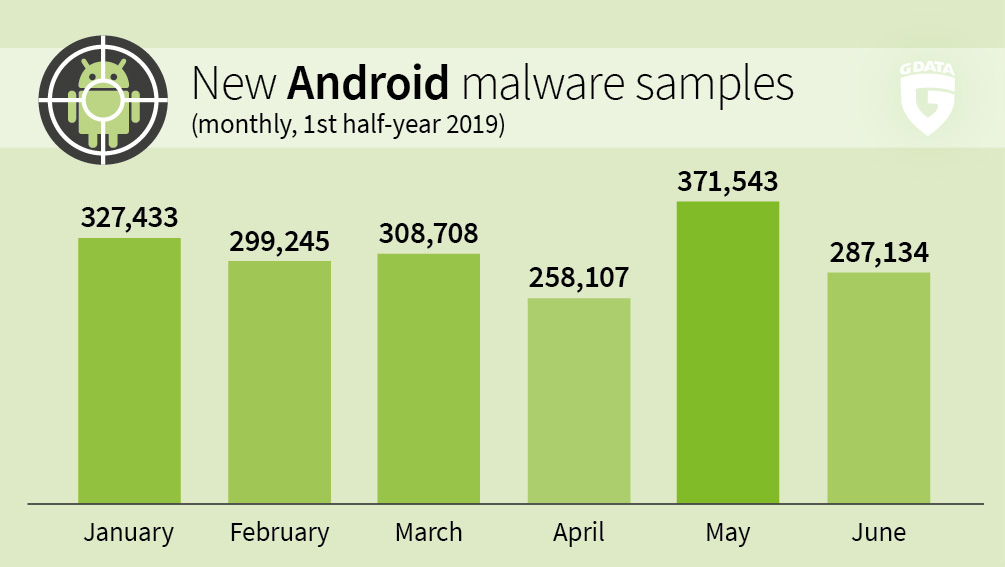
\includegraphics[width=0.6\textwidth]{imgs/capitolo3/G_DATA-Infographic-MMR-HJ1-2019-New_Android_Malware-monthly-EN-Logo.jpg}
        \caption{Malware detection 2019 - G DATA}
        \label{fig:GSATA}
\end{figure}
\FloatBarrier %  evitare che i float appaiano oltre un certo punto nel tuo documento %
\begin{figure}[h]
        \centering
        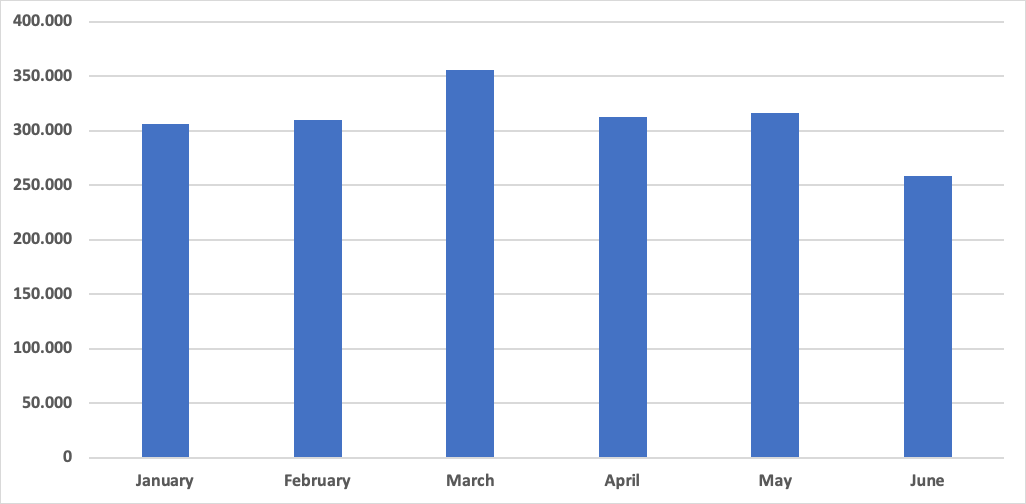
\includegraphics[width=0.6\textwidth]{imgs/capitolo3/avira.png}
        \caption{malware detection 2020 - Avira}
        \label{fig:avira}
        \end{figure}
\FloatBarrier %  evitare che i float appaiano oltre un certo punto nel tuo documento %
Il malware inoltre è stato la categoria di malware che più è stata rilevata come minaccia in ambiente andorid, quasi $3/4$ delle rilevazioni riguardavano appunto un malware\cite{newMalwareAvira}.
Questo è stato reso possibile dalla frammentazione del mercato. Essendo un sistema operativo in continua evoluzione e diffusione diventa sempre più complesso riuscire a garantire la sicurezza di tutte le versioni in circolazione. Di fatti un problema per la sicurezza è legato alla versione android istallata sul proprio device. Nel 2017 si stimava ci fossero circa 1 miliardo di dispositivi android che non fossero aggiornati o non avrebbero ricevuto aggiornamenti, rendendo i dispositivi sempre più obsoleti e vulnerabili\cite{oneMilion}. 

In figura \ref{fig:os version}, nell'intervallo che va dal Gennaio 2019 al Gennaio 2021 possiamo infatti osservare come le due versioni più diffuse siano Android 9 (2017) e Andorid 8 (2018) 

    \begin{figure}[h]
        \centering
        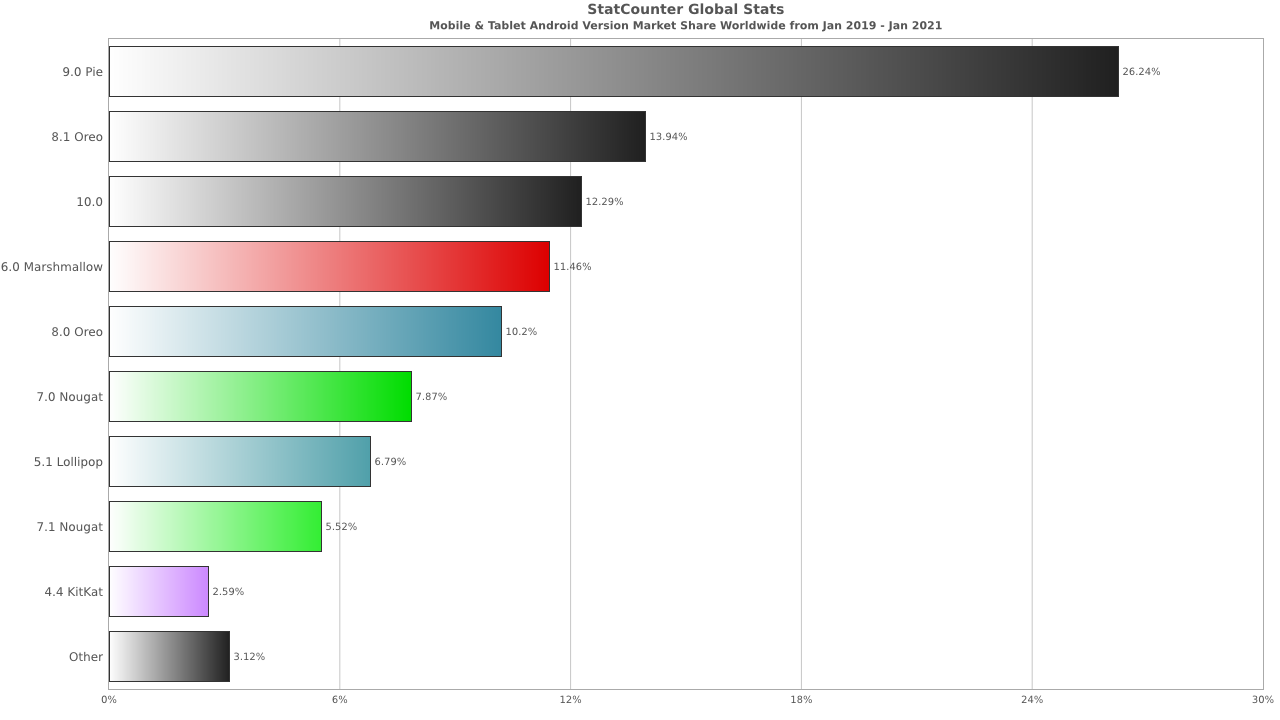
\includegraphics[width=0.6\textwidth]{imgs/capitolo3/StatCounter-android_version-ww-monthly-201901-202101-bar.png}
        \caption{Android OS Version - GlobalStats statcounter}
        \label{fig:os version}
        \end{figure}
        \FloatBarrier %  evitare che i float appaiano oltre un certo punto nel tuo documento %


Il rischio rimane quindi molto alto e da non sottovalutare. 
Nel prossimo paragrafo vedremo cosa si intende per malware. 
\section{Malware}
un Malicius software abbreviato, Malware, è un termine che va ad indicare tutti quei programmi che mettono a rischio un sistema informatico. La maggior diffusione avviene attraverso internet e più nello specifico attraverso le e-mail, in ambiente mobile però le app dannose possono nascondersi anche all'interno di applicazioni che all'apparenza sembrano non rappresentare una minaccia, questo avviene soprattutto se ci si affida per il download a store non ufficiali. I tipi di malware più diffusi sono: 
\begin{itemize}
    \item \textit{Virus}: programmi presenti in applicazini che una volta eseguite diffondono il codice malevole ad altri programmi del sistema;
    \item \textit{Trojan}: codice che solitamente è nascosto in applicazioni che riusltano utili all'utente ma che una volta istallate consentono agli attaccanti di ottenere l'accesso al dispositivo; 
    \item \textit{Ransomware}: impediscono all'utente di accedere al proprio dispositivo cifrando i suoi file, spesso sono seguiti da una richiesta di riscatto a pagare un riscatto per riottenere l'accesso al dispositivo; 
    \item \textit{Worm} si diffondono nei dispositivi di una rete danneggiandoli mediante la distruzione di dati e file;
\end{itemize}

Da un'indaggine condotta da AV-Test, i trojan sono risultati il mezzo preferito dai criminali informatici per introdurre codice malevolo rappresentando il 93.93\%  di tutti gli attacchi di malware sui sistemi Android. Il ransomware si è classificato al secondo posto, con il 2,47\% \cite{trojan}.

\subsection{Covert Channel}
\textbf{TODO: Parlare die covert channel?}